documentclass[tikz,border=2mm]{standalone}
\begin{document}

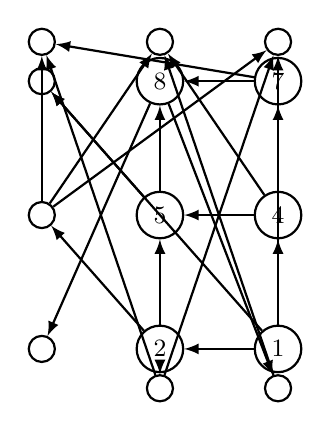
\begin{tikzpicture}[node distance={25mm}, thick]
\draw (-1.5,-1.7) node(A) [shape=circle,draw=black,fill=white]{\small 1};
\draw (-1.5,0) node(B) [shape=circle,draw=black,fill=white]{\small 4};
\draw (-1.5,1.7) node(C) [shape=circle,draw=black,fill=white]{\small 7};
\draw (-3,-1.7) node(D) [shape=circle,draw=black,fill=white]{\small 2};
\draw (-3,0) node(E) [shape=circle,draw=black,fill=white]{\small 5};
\draw (-3,1.7) node(F) [shape=circle,draw=black,fill=white]{\small 8};
\draw (-1.5,-2.2) node(G) [shape=circle,draw=black,fill=white]{};
\draw (-3,-2.2) node(H) [shape=circle,draw=black,fill=white]{};
\draw (-4.5,0) node(I) [shape=circle,draw=black,fill=white]{};
\draw (-4.5,1.7) node(J) [shape=circle,draw=black,fill=white]{};
\draw (-4.5,-1.7) node(K) [shape=circle,draw=black,fill=white]{};
\draw (-1.5,2.2) node(L) [shape=circle,draw=black,fill=white]{};
\draw (-3,2.2) node(M) [shape=circle,draw=black,fill=white]{};
\draw (-4.5,2.2) node(N) [shape=circle,draw=black,fill=white]{};

\draw [-latex] (A) edge (B);
\draw [-latex] (B) edge (C);
\draw [-latex] (D) edge (E);
\draw [-latex] (E) edge (F);
\draw [-latex] (A) edge (D);
\draw [-latex] (B) edge (E);
\draw [-latex] (C) edge (F);
\draw [-latex] (A) edge (L);
\draw [-latex] (B) edge (M);
\draw [-latex] (C) edge (N);
\draw [-latex] (D) edge (I);
\draw [-latex] (E) edge (J);
\draw [-latex] (F) edge (K);
\draw [-latex] (A) edge (J);
\draw [-latex] (D) edge (H);
\draw [-latex] (F) edge (G);
\draw [-latex] (H) edge (L);
\draw [-latex] (G) edge (M);
\draw [-latex] (H) edge (N);
\draw [-latex] (I) edge (L);
\draw [-latex] (I) edge (M);
\draw [-latex] (I) edge (N);
\end{tikzpicture}

\end{document}